\documentclass{report}
% Include all project wide packages here.
\usepackage{fullpage}
\usepackage[style=ieee]{biblatex}
\usepackage[dutch]{babel}

\renewcommand{\familydefault}{\sfdefault}

\setmainfont[Ligatures=TeX]{Myriad Pro}
\setmathfont{Asana Math}
\setmonofont{Lucida Console}

\usepackage{titlesec, blindtext, color}
\definecolor{gray75}{gray}{0.75}
\newcommand{\hsp}{\hspace{20pt}}
\titleformat{\chapter}[hang]{\Huge\bfseries}{\thechapter\hsp\textcolor{gray75}{|}\hsp}{0pt}{\Huge\bfseries}
\renewcommand{\familydefault}{\sfdefault}
\renewcommand{\arraystretch}{1.2}
\setlength\parindent{0pt}

%For code listings
\definecolor{black}{rgb}{0,0,0}
\definecolor{browntags}{rgb}{0.65,0.1,0.1}
\definecolor{bluestrings}{rgb}{0,0,1}
\definecolor{graycomments}{rgb}{0.4,0.4,0.4}
\definecolor{redkeywords}{rgb}{1,0,0}
\definecolor{bluekeywords}{rgb}{0.13,0.13,0.8}
\definecolor{greencomments}{rgb}{0,0.5,0}
\definecolor{redstrings}{rgb}{0.9,0,0}
\definecolor{purpleidentifiers}{rgb}{0.01,0,0.01}


\lstdefinestyle{csharp}{
language=[Sharp]C,
showspaces=false,
showtabs=false,
breaklines=true,
showstringspaces=false,
breakatwhitespace=true,
escapeinside={(*@}{@*)},
columns=fullflexible,
commentstyle=\color{greencomments},
keywordstyle=\color{bluekeywords}\bfseries,
stringstyle=\color{redstrings},
identifierstyle=\color{purpleidentifiers},
basicstyle=\ttfamily\small}

\lstdefinestyle{c}{
language=C,
showspaces=false,
showtabs=false,
breaklines=true,
showstringspaces=false,
breakatwhitespace=true,
escapeinside={(*@}{@*)},
columns=fullflexible,
commentstyle=\color{greencomments},
keywordstyle=\color{bluekeywords}\bfseries,
stringstyle=\color{bluestrings},
identifierstyle=\color{purpleidentifiers}
}

\lstdefinestyle{vhdl}{
language=VHDL,
showspaces=false,
showtabs=false,
breaklines=true,
showstringspaces=false,
breakatwhitespace=true,
escapeinside={(*@}{@*)},
columns=fullflexible,
commentstyle=\color{greencomments},
keywordstyle=\color{bluekeywords}\bfseries,
stringstyle=\color{redstrings},
identifierstyle=\color{purpleidentifiers}
}

\lstdefinestyle{xaml}{
language=XML,
showspaces=false,
showtabs=false,
breaklines=true,
showstringspaces=false,
breakatwhitespace=true,
escapeinside={(*@}{@*)},
columns=fullflexible,
commentstyle=\color{greencomments},
keywordstyle=\color{redkeywords},
stringstyle=\color{bluestrings},
tagstyle=\color{browntags},
morestring=[b]",
  morecomment=[s]{<?}{?>},
  morekeywords={xmlns,version,typex:AsyncRecords,x:Arguments,x:Boolean,x:Byte,x:Char,x:Class,x:ClassAttributes,x:ClassModifier,x:Code,x:ConnectionId,x:Decimal,x:Double,x:FactoryMethod,x:FieldModifier,x:Int16,x:Int32,x:Int64,x:Key,x:Members,x:Name,x:Object,x:Property,x:Shared,x:Single,x:String,x:Subclass,x:SynchronousMode,x:TimeSpan,x:TypeArguments,x:Uid,x:Uri,x:XData,Grid.Column,Grid.ColumnSpan,Click,ClipToBounds,Content,DropDownOpened,FontSize,Foreground,Header,Height,HorizontalAlignment,HorizontalContentAlignment,IsCancel,IsDefault,IsEnabled,IsSelected,Margin,MinHeight,MinWidth,Padding,SnapsToDevicePixels,Target,TextWrapping,Title,VerticalAlignment,VerticalContentAlignment,Width,WindowStartupLocation,Binding,Mode,OneWay,xmlns:x}
}

%defaults
\lstset{
basicstyle=\ttfamily\small,
extendedchars=false,
numbers=left,
numberstyle=\ttfamily\tiny,
stepnumber=1,
tabsize=4,
numbersep=5pt
}

\begin{document}
\chapter{Methode}
\section{Benodigdheden}
De benodigdheden zijn als volgt:
\begin{itemize}
\item EPO-2 robot met de juiste programmatuur in de ROM van het FPGA bord
\item Papier met kalibratielijnen en lijnen op onbekende afstand van elkaar
\item Liniaal
\end{itemize}
\section{Handelswijze}
Eerst laat men de robot de kalibratieafstand tien keer meten. Dit wordt gedaan door de robot voor de eerste lijn op het kalibratiepapier (Figuur \ref{fig:testSheets}) te zetten en dan op de startknop (button 1) te drukken. Het is het beste om hierbij de voorkant van de robot tegen de grond te houden, anders komt de reflectiesensor te ver omhoog om de grond nog waar te kunnen nemen. De robot stopt vanzelf als hij de overkant heeft bereikt en geeft dan de verstreken tijd weer tussen het doorkruisen van de start- en eindlijn. Het aflezen gaat in 2 stappen; de robot weergeeft eerst de eerste vier cijfers en dan de laatste vier cijfers, op deze manier: $XX.XXYYYY$. Of de robot de eerste set of tweede set cijfers weergeeft is te zien aan het al dan niet ontbreken van een decimale punt. 
\begin{figure}[H]
\includegraphics[width=0.33\textwidth,page=2]{test_sheets_A3-rc.pdf}
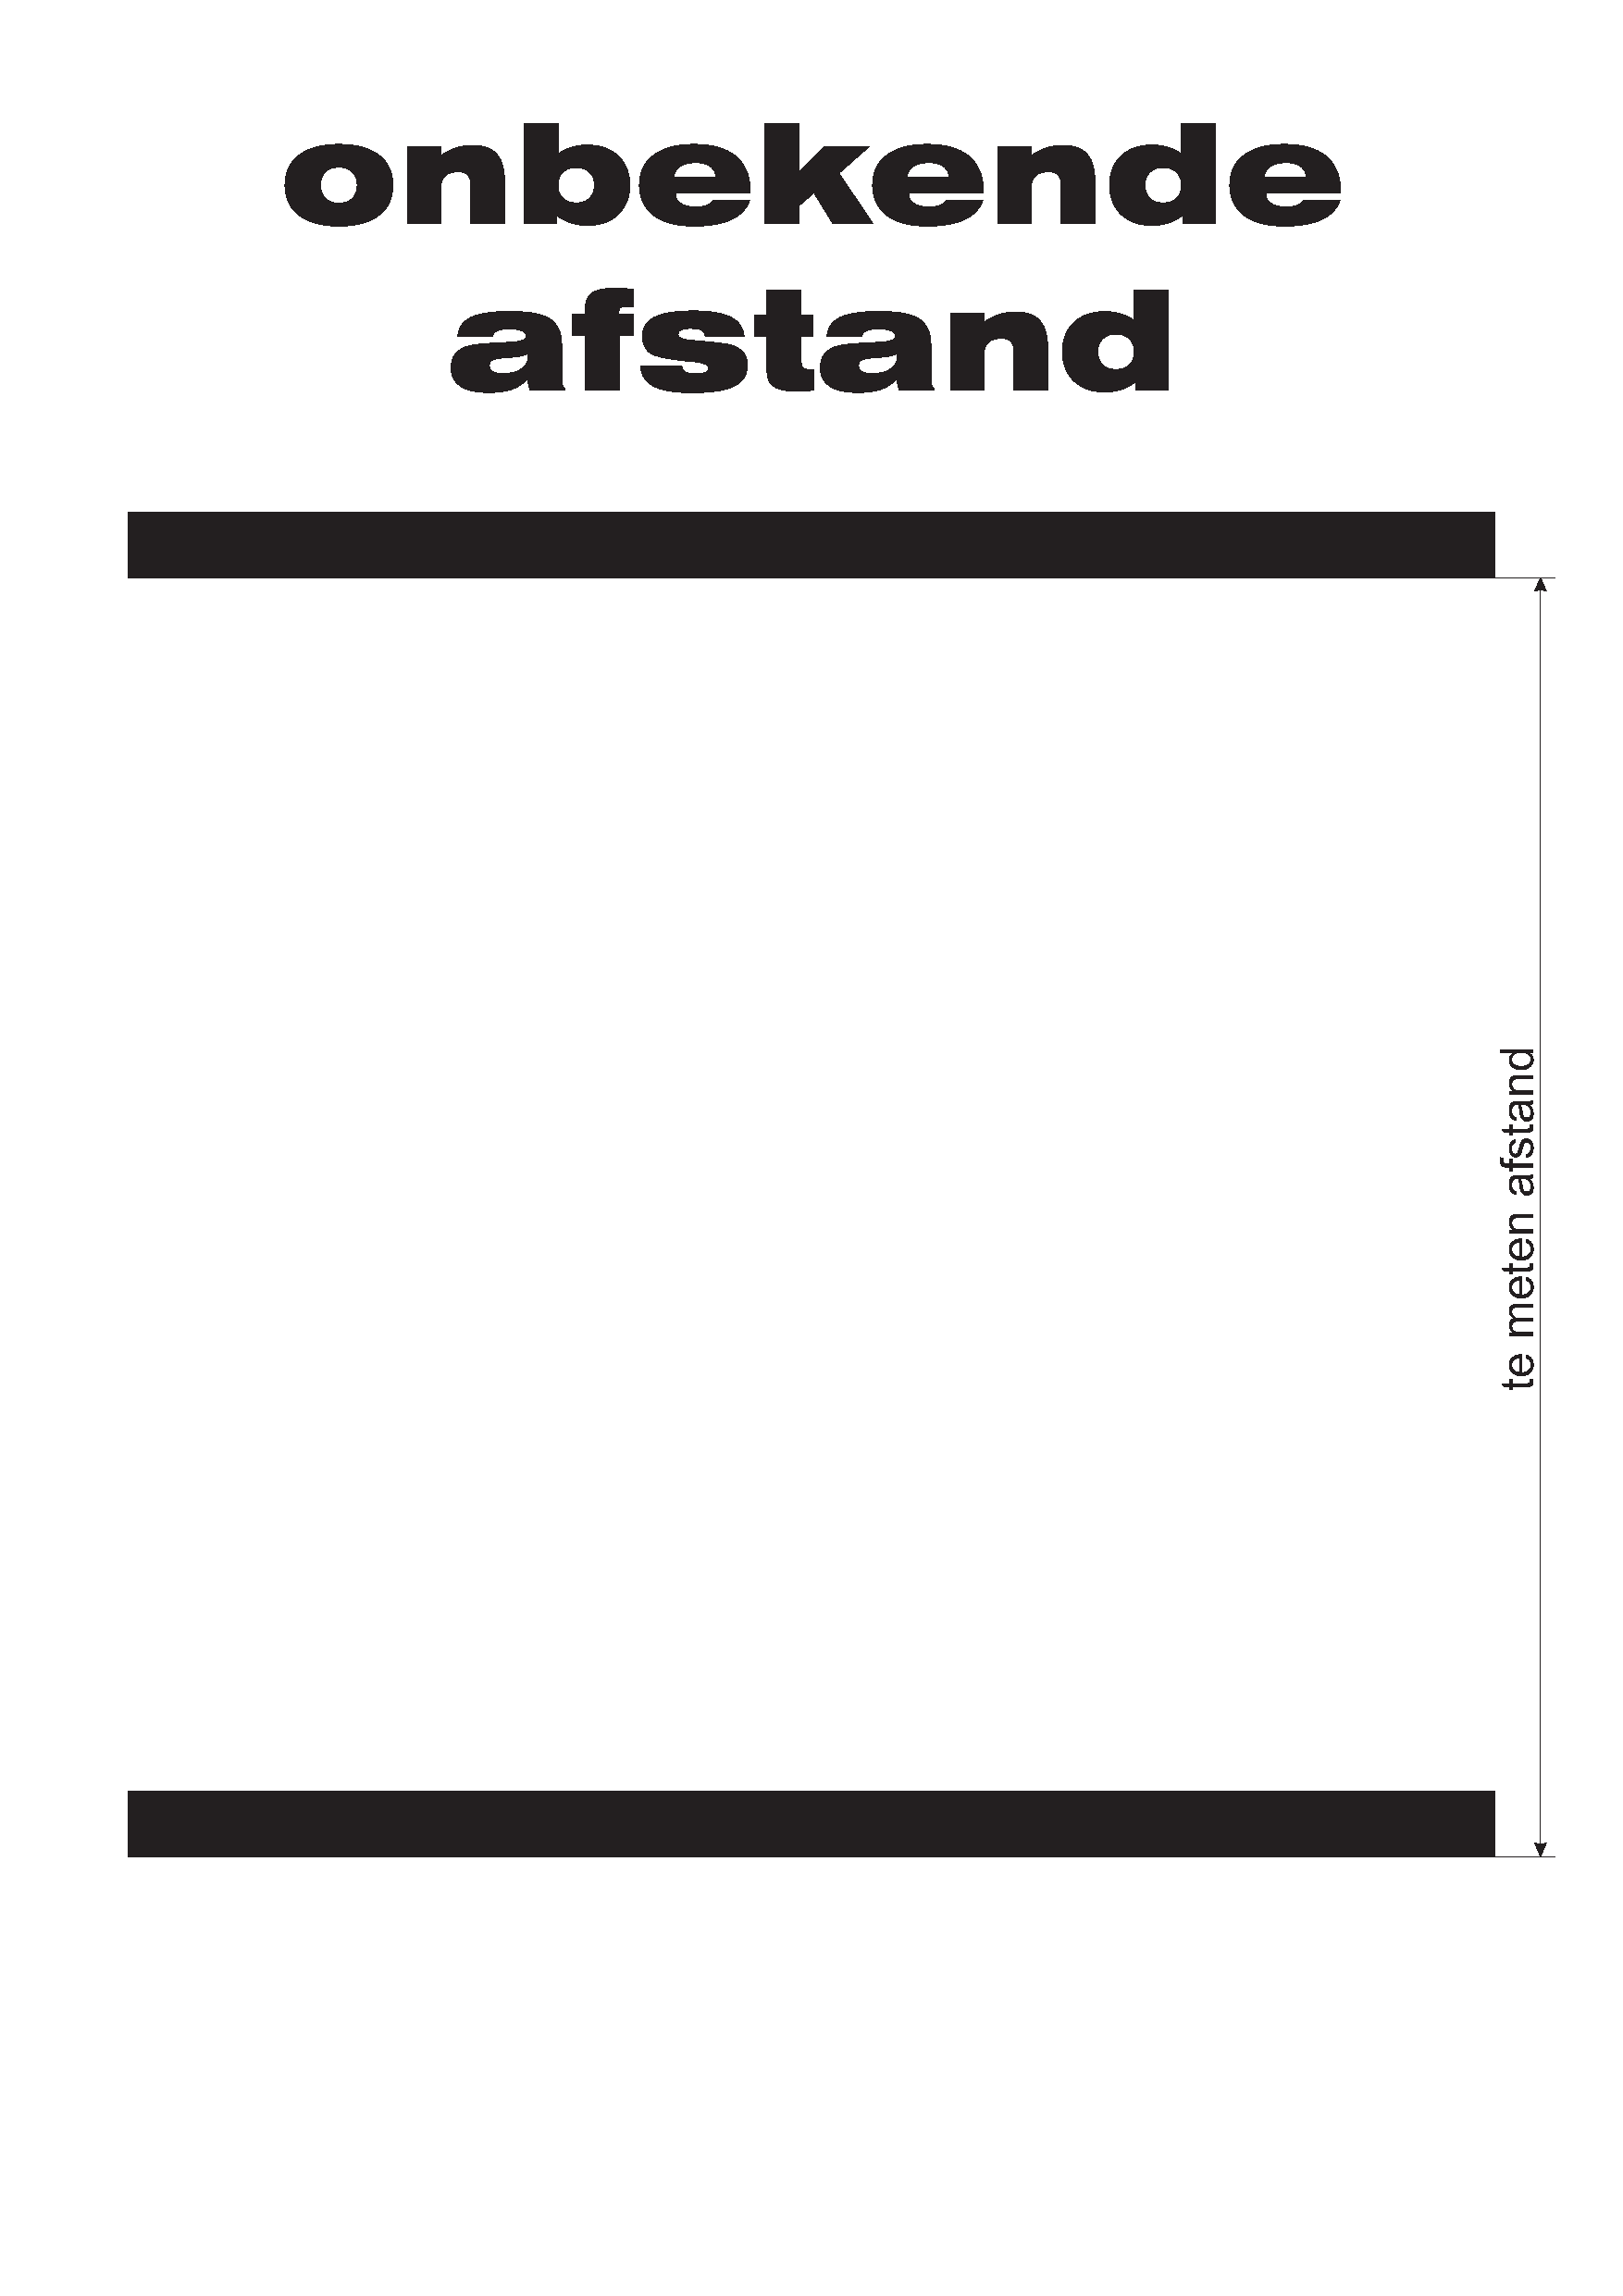
\includegraphics[width=0.33\textwidth,page=1]{test_sheets_A3-rc.pdf}
\includegraphics[width=0.33\textwidth,page=3]{test_sheets_A3-rc.pdf}
\caption{De test sheets}
\label{fig:testSheets}
\end{figure}
De robot die wij hebben gebruikt had een afwijking naar links. Hij maakte een cirkel met een straal tussen de 0.8 en 1 meter, als de afstand die gemeten moet worden vrij lang is moet de robot dus op zodanige wijze voor de eerste lijn gepositioneerd worden dat hij goed uit komt op de tweede.

Na de kalibratie, waaruit de gemiddelde snelheid van de robot kan worden bepaald middels $v=\frac{s}{t}$, kunnen de overige metingen met onbekende afstanden worden uitgevoerd zoals beschreven in de handleiding. Aan de hand van die resultaten kunnen de onbekende afstanden bepaald worden met $s=vt$. Elke meting zou zo'n tien maal gedaan kunnen worden voor een nauwkeuriger eindresultaat.
\end{document}